%% LyX 2.1.4 created this file.  For more info, see http://www.lyx.org/.
%% Do not edit unless you really know what you are doing.
\documentclass{UNCC-thesis}
\usepackage[T1]{fontenc}
\usepackage[latin9]{inputenc}
\setcounter{secnumdepth}{3}
\usepackage{array}
\usepackage{float}
\usepackage{graphicx}
\usepackage{nomencl}
% the following is useful when we have the old nomencl.sty package
\providecommand{\printnomenclature}{\printglossary}
\providecommand{\makenomenclature}{\makeglossary}
\makenomenclature

\makeatletter

%%%%%%%%%%%%%%%%%%%%%%%%%%%%%% LyX specific LaTeX commands.
%% Because html converters don't know tabularnewline
\providecommand{\tabularnewline}{\\}

%%%%%%%%%%%%%%%%%%%%%%%%%%%%%% User specified LaTeX commands.
% If you are using MikTeX on Windows and you have a nomenclature section
% you may want to uncomment the line below.
%
%\immediate\write18{makeindex msthesis.nlo -s nomencl.ist -o msthesis.nls}

\@ifundefined{showcaptionsetup}{}{%
 \PassOptionsToPackage{caption=false}{subfig}}
\usepackage{subfig}
\makeatother

\begin{document}
\pagenumbering{roman}
\fbmatterchapterformat
% Doctype should be either dissertation proposal, dissertation, or thesis.
% If you're getting a master's, specify "thesis" below.  
% If you're getting a PhD, specify "dissertation" below.
\doctype{thesis}
%%%%%%%%%%%%%%%%     IMPORTANT! IMPORTANT! IMPORTANT! %%%%%%%%%%%%%%%%
% The rules below MUST be followed for the abstract page and chapter titles
% to be correctly formatted.
%
% 1. Only the first letter of the entire title should be capitalized to allow the 
%    title to appear as required by the graduate school on the Abstract page.
% 2. Write chapter titles in ALL CAPS.
%
\title{My lyx thesis}
\author{Test User}
\degree{Master of Science}
\major{Electrical Engineering}
\publicationyear{2015}

\advisor{Dr. Person A}

% Add the full name and title of all your committee members,
% apart from your advisor, one by one.  The style file expects
% 3 to 5 committee members in addition to your advisor.

\committeeMember{Dr. Person B}
\committeeMember{Dr. Person C}


% Generate the preliminary title page and copyright page.
\maketitlepage
\makecopyright
\begin{abstract}
You must have an abstract. The content of your abstract goes here. 

You should compose the abstract using the conventions of your field. In many fields this section is typically 1-2 pages. \end{abstract}
\begin{dedication}
If you decide to have a dedication page, your dedication text would
go here.

The Dedication page, if used, pays a special tribute to a person(s)
who has given extraordinary encouragement or support to one's academic
career.\end{dedication}
\begin{acknowledgements}
If you decide to have a acknowledgements page, your acknowledgement
text would go here.

The Acknowledgement page should be brief, simple, and free of sentimentality
or trivia. It is customary to recognize the role of the advisor, the
other members of the advisory committee, and only those organizations
or individuals who actually aided in the project. Further, you should
acknowledge any outside source of financial assistance, such as GASP
grants, contracts, or fellowships.
\end{acknowledgements}
\tableofcontents{}

\listoftables


\listoffigures


\newpage
\renewcommand{\nomname}{LIST OF ABBREVIATIONS}
% uncomment line below to title your nomenclature list as LIST OF SYMBOLS
%\renewcommand{\nomname}{LIST OF SYMBOLS}
%
% NOTE: IF YOU USE A LIST OF ABBREVIATIONS / LIST OF SYMBOLS and are using command-line LaTeX (not LyX) 
% YOU MUST COMPILE THE NOMENCLATURE INDEX
% example:
% bash$> pdflatex msthesis.tex
% bash$> makeindex msthesis.nlo -s nomencl.ist -o msthesis.nls
% bash$> pdflatex msthesis.tex
%
\addcontentsline{toc}{chapter}{\nomname}\settowidth{\nomlabelwidth}{ECE}
\printnomenclature{}

\nomenclature{ECE}{An acronym for Electrical and Computer Engineering.}

\newpage
\setcounter{page}{1}
\pagenumbering{arabic}
% 2 inch top spacing for new chapters
\bodychapterformat
\begin{preface}
If you decide to have an introduction page, your introduction text
would go here. 

Depending on the discipline or the requirements of the student's advisory
committee, an Introduction may be included as a preliminary page.
\end{preface}

\chapter{INTRODUCTION}

This is my introduction. Here is an example of a citation using BiB\TeX{}
that cites the GNU project, a major force in free software advocacy
\cite{gpl}. The UNC Charlotte thesis guidelines state the following
about the text of thesis and dissertation documents:
\begin{quote}
``Do not use bold, underline or create unusual fonts for chapter
titles; do not use running headers or footers. Do not use bold, underline
or italics for headings, subheadings, etc. Changes in font style or
typeface are not permitted except for inclusion of illustrative or
documentary materials such as computer printouts or if required for
mathematical expressions. If you are unsure about the acceptability
of the typeface you want to use for your final copy of the thesis
or dissertation, please verify with the thesis/dissertation reviewer
in the Graduate School that it can be used.'' \emph{--~UNC Charlotte
Guidelines 2014: Thesis Text} (page 4)
\end{quote}
\begin{table}[H]
\begin{centering}
{\small{}}%
\begin{tabular}{|c|>{\centering}p{1in}|>{\centering}p{1in}|>{\centering}p{1in}|>{\centering}p{1in}|}
\hline 
{\small{}Case \#} & {\small{}Translational displcmnt.} & {\small{}Total $\alpha$} & {\small{}Total $\beta$} & {\small{}Total $\gamma$ }\tabularnewline
\hline 
\hline 
{\small{}6} & {\small{}83.09} & {\small{}885.66} & {\small{}252.07} & {\small{}264.64}\tabularnewline
\hline 
{\small{}7} & {\small{}63.12} & {\small{}337.48} & {\small{}244.95} & {\small{}381.31}\tabularnewline
\hline 
{\small{}8} & {\small{}70.45} & {\small{}240.08} & {\small{}217.59} & {\small{}294.56}\tabularnewline
\hline 
{\small{}12} & {\small{}15.71} & {\small{}86.89} & {\small{}74.58} & {\small{}112.03}\tabularnewline
\hline 
\end{tabular}
\par\end{centering}{\small \par}

\caption{\label{tab:Table1}This is an example of a table.}
\end{table}



\section{Problem Statement}

This is an example of a subsection. I have included Table \ref{tab:Table1}
and Table \ref{tab:Table2} as examples of how to place tables and
table cross-references in your document. I have also included Figure
\ref{fig:LinearFit} which has subfigures within it to provide an
example of a graphical figure in the document. Labeling tables and
figures and cross-referencing these labels in your text will ensure
that the list of figures and list of tables generated automatically
will always be correct even when you move figures and tables to new
locations in your document. 
\begin{table}[H]
\centering{}{\small{}}%
\begin{tabular}{|>{\centering}p{1in}|>{\centering}p{1in}|>{\centering}p{1in}|}
\hline 
{\small{}R} & {\small{}Overall severity} & {\small{}KL-score}\tabularnewline
\hline 
\hline 
{\small{}Translation} & {\small{}0.68} & {\small{}0.28}\tabularnewline
\hline 
{\small{} $\alpha$} & {\small{}0.34} & {\small{}0.17}\tabularnewline
\hline 
{\small{}$\beta$} & {\small{}0.59} & {\small{}0.27}\tabularnewline
\hline 
{\small{}$\gamma$} & {\small{}0.53} & {\small{}0.29}\tabularnewline
\hline 
\end{tabular}\caption[Example of short label.]{\label{tab:Table2}This is an example of a table having a long caption
whose caption in the list of tables is much shorter (from the ``opt''
label). Correlation coefficient (R) comparison between displacement
parameters and average overall ranking and KL score.}
\end{table}
\begin{figure}[H]
\begin{centering}
\subfloat[Translational displacement vs. Savg; a linear fit ]{\begin{centering}
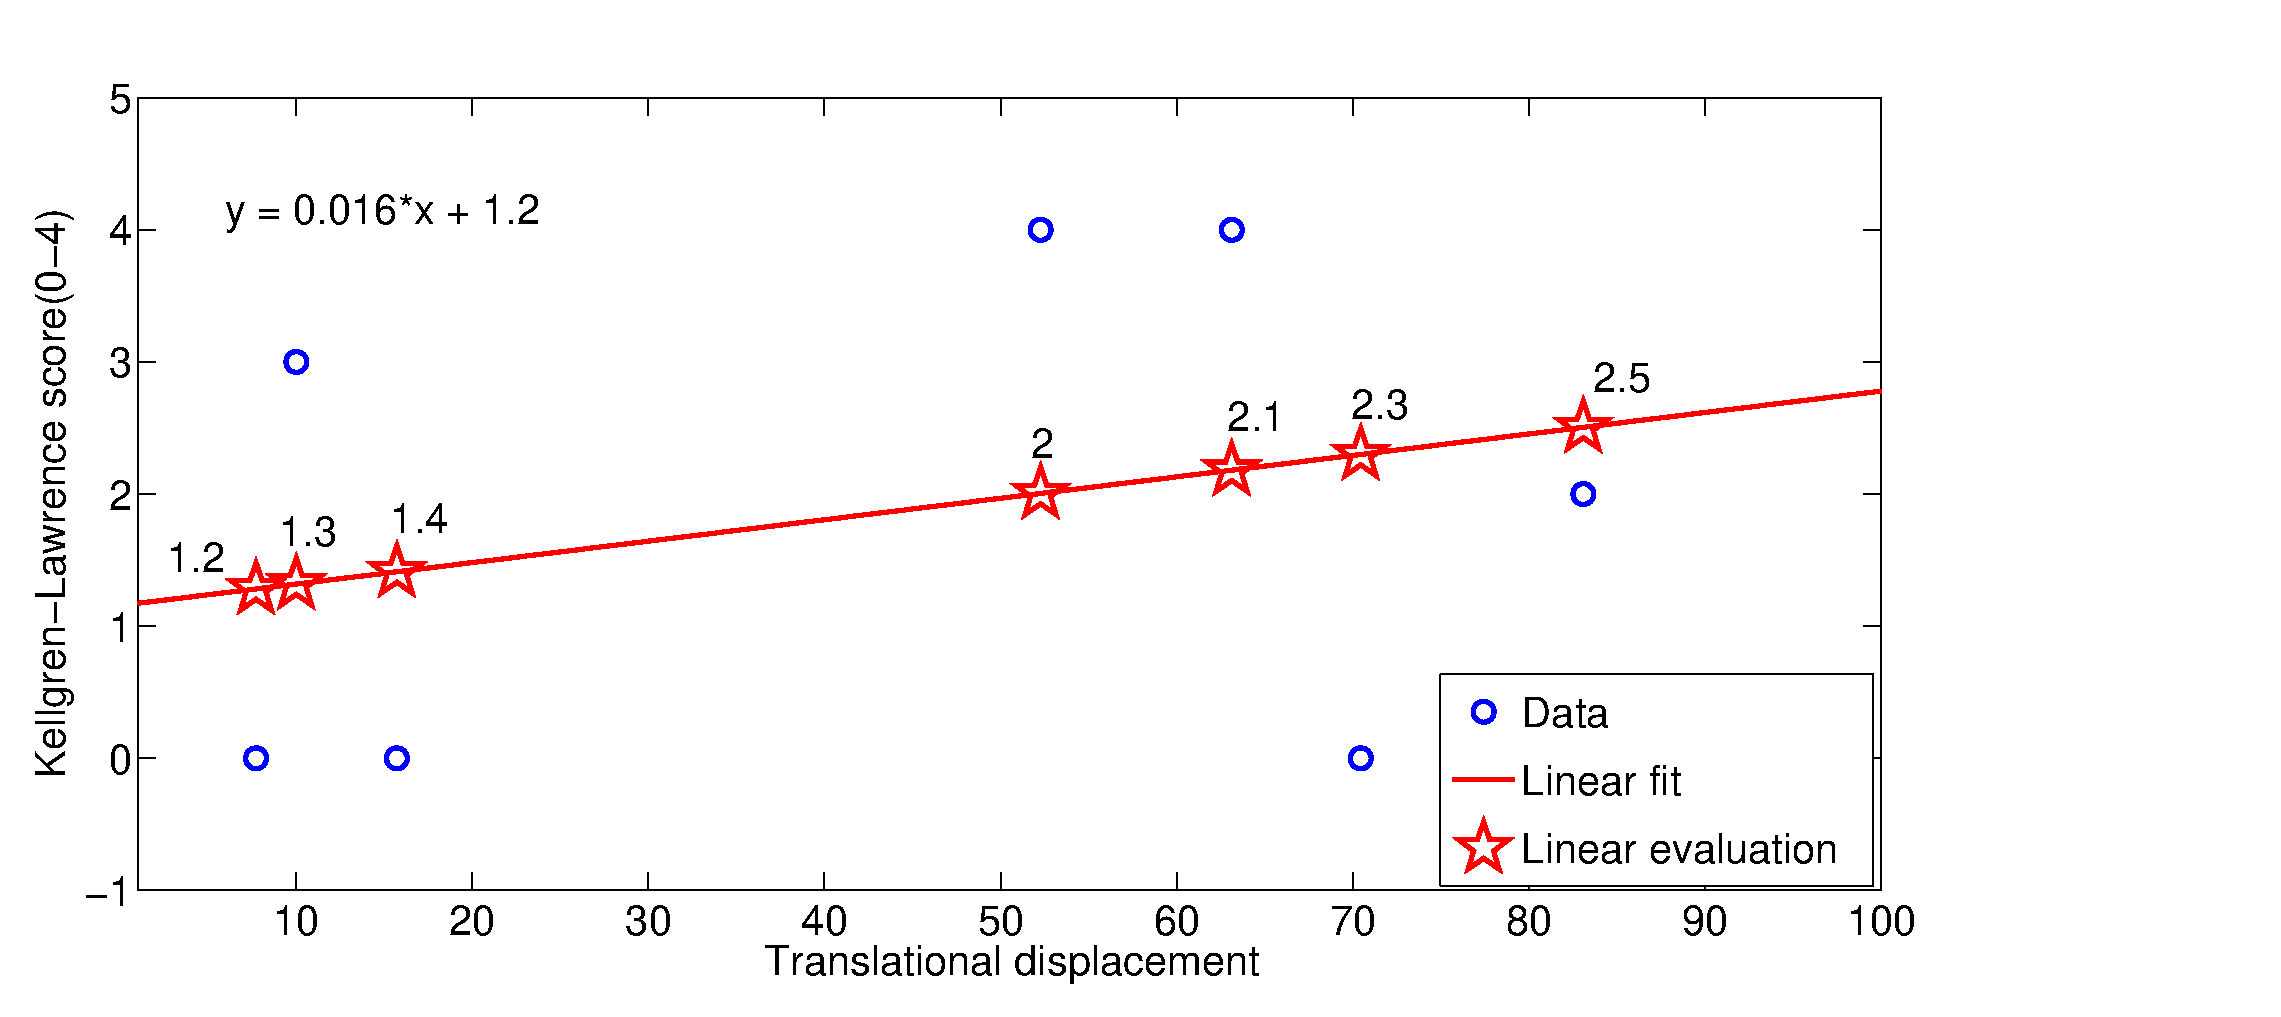
\includegraphics[height=2in]{figs/TransVsKLLine}
\par\end{centering}

}
\par\end{centering}

\begin{centering}
\subfloat[Translational displacement vs. KL; a linear fit ]{\begin{centering}
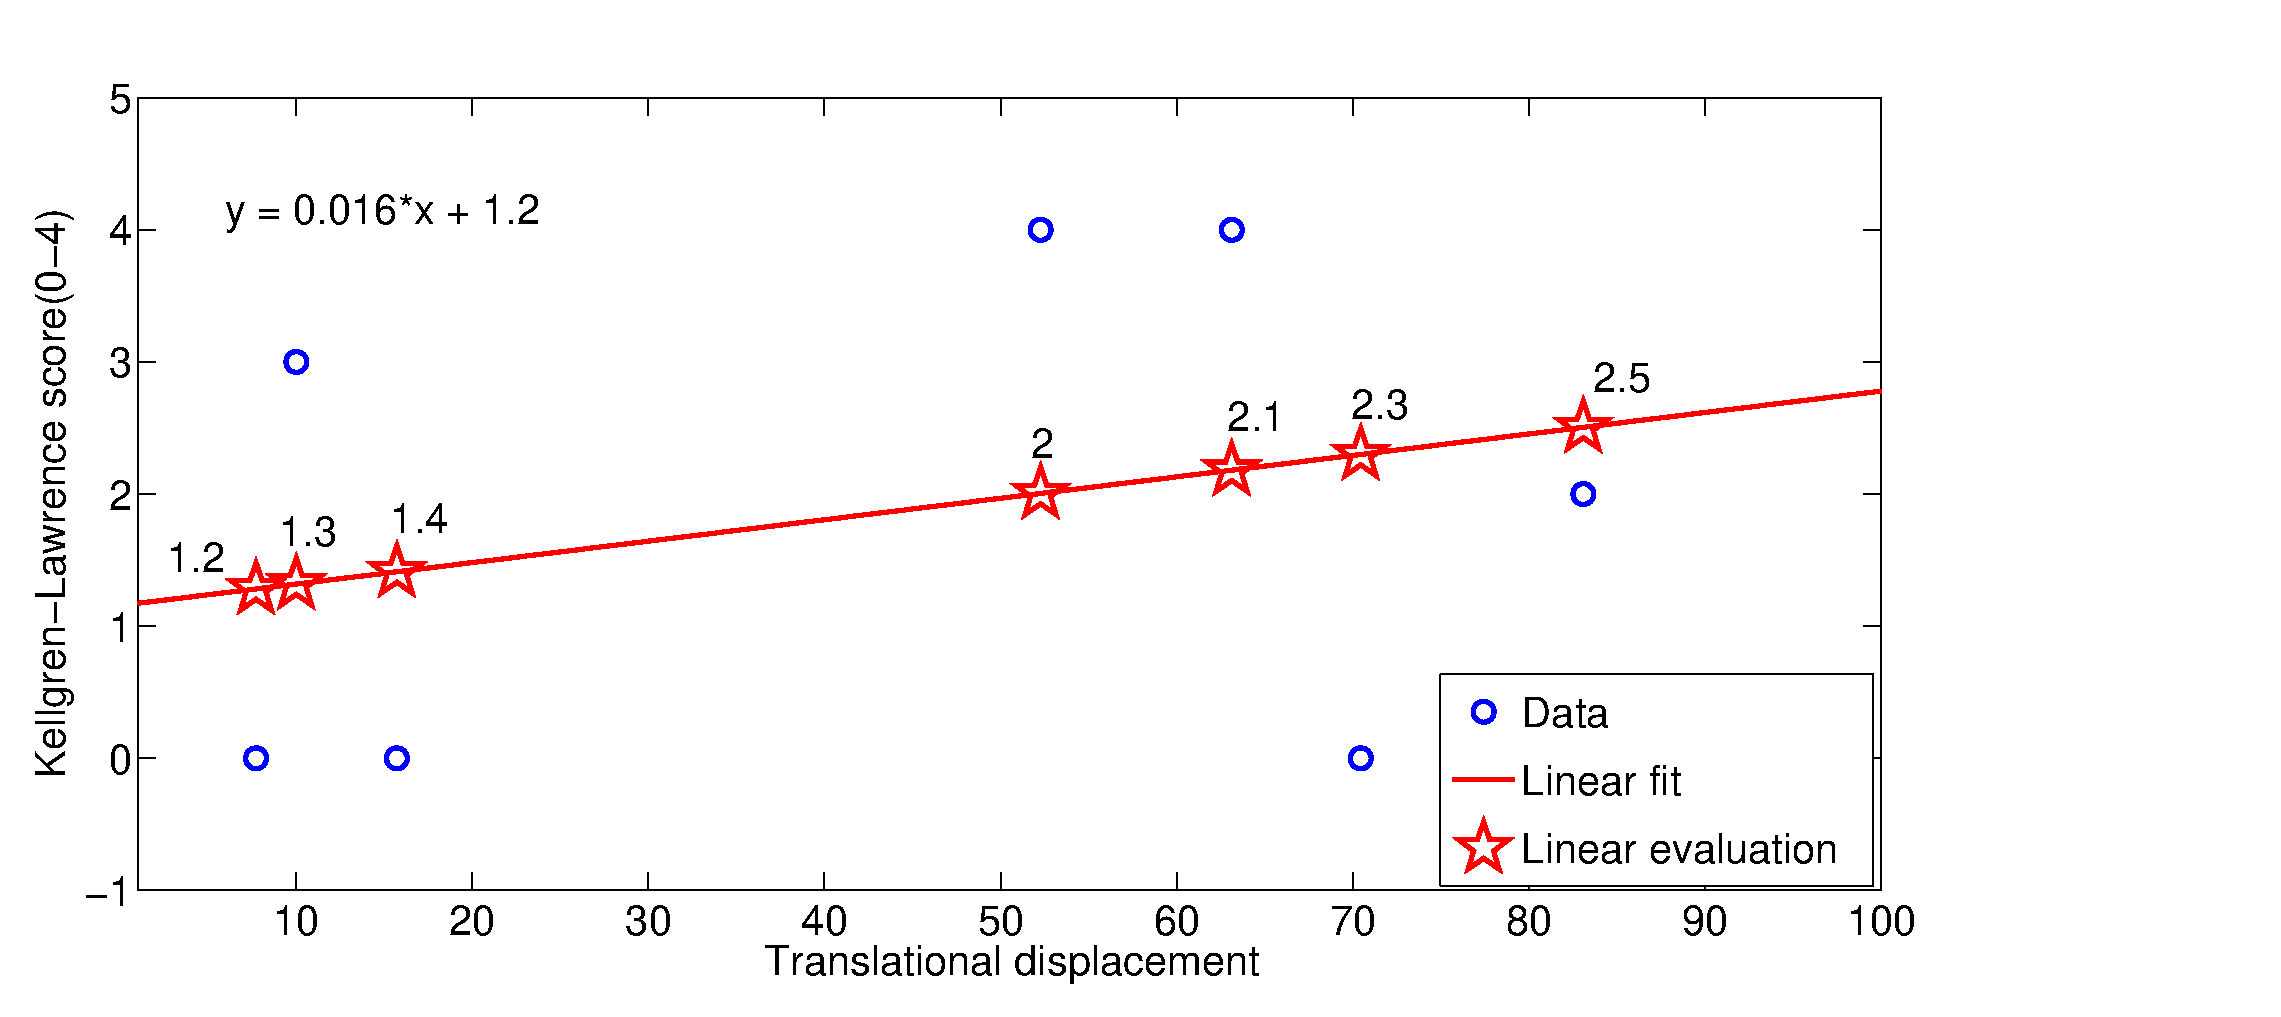
\includegraphics[height=2in]{figs/TransVsKLLine}
\par\end{centering}

}
\par\end{centering}

\caption[Shortened figure caption for list of figures.]{\label{fig:LinearFit}Linear fitting translational displacement to
KL and average overall severity.}
\end{figure}



\chapter{CONCLUSIONS}

Lots of interesting conclusions will be put here.

\fbmatterchapterformat

\bibliographystyle{ieeetr}
\bibliography{references_db}


\newpage{}\uncctocformat{chapter}{0pt}{350pt}{\appendixname~\thecontentslabel:~}
\renewcommand{\chaptertitlename}{APPENDIX}
%
% The default setting for appendices excludes sections, subsections, etc. from
% the TABLE OF CONTENTS.
% If you want these in the TABLE OF CONTENTS, increase the number in the line below:
% 1 - Appendices, Sections / 2 - Appendices, Sections, Subsections / 3 - etc 
%
\addtocontents{toc}{\protect\setcounter{tocdepth}{0}}

\appendix

\chapter{QUADRATIC FIT COMPARISON GRAPHS}

The appendices should be used for whatever material you or your advisory
committee believes should be included, but would not be appropriate
in the text of the thesis or dissertation. Such materials can include:
\begin{enumerate}
\item the original data obtained in the thesis or dissertation research,
including computer programs and printouts, surveys, or correspondence;
\item detailed descriptions of procedures, which go beyond the general outline
of methods and approaches presented in the text;
\item a particularly extensive review of the literature and other information
that may be useful to future scholars who may wish to delve more deeply
into the research topic.
\end{enumerate}

\section{Section in appendix}

This is a section in the appendix.
\end{document}
